%\documentclass{emulateapj} %astro-ph
\documentclass[10pt,preprint]{aastex} %ApJ
\usepackage{graphicx}
\usepackage{color,calc}
%\usepackage{natbib}
\usepackage{amsmath}
\usepackage{amssymb}
\usepackage{amstext}
\usepackage{moreverb}
%\usepackage{pstricks}
%\usepackage{pst-node}
%\usepackage{pst-tree}

%%%%%%%%%%%%%%%%%%%%%%%%%%%%%%%%%%%%%%%%%%%%%%%%%%%%%%%%%%%%%%%%%%%%%%%%%%%%%%%
\newcommand{\note}[3]{{\color{red}\bf [#1: #2 -- #3]}}
\newcommand{\Fewbody}{{\em Fewbody\/}}
\newcommand{\GLStarView}{{\em GLStarView\/}}
\newcommand{\Starlab}{{\em Starlab\/}}
\newcommand{\hier}{{\tt hier}}
\newcommand{\obj}{{\tt obj}}

%%%%%%%%%%%%%%%%%%%%%%%%%%%%%%%%%%%%%%%%%%%%%%%%%%%%%%%%%%%%%%%%%%%%%%%%%%%%%%%
\begin{document}

%%%%%%%%%%%%%%%%%%%%%%%%%%%%%%%%%%%%%%%%%%%%%%%%%%%%%%%%%%%%%%%%%%%%%%%%%%%%%%%
\title{Fewbody: A Brief Developer's Guide}
\shorttitle{Fewbody}
%\submitted{Documentation}
\author{John M. Fregeau}
\shortauthors{FREGEAU}
\affil{Kavli Institute for Theoretical Physics, UCSB, Santa Barbara, CA 93106, USA}

%%%%%%%%%%%%%%%%%%%%%%%%%%%%%%%%%%%%%%%%%%%%%%%%%%%%%%%%%%%%%%%%%%%%%%%%%%%%%%%
\begin{abstract}
This document serves as a brief guide for those who want to use \Fewbody\ through
its C interface.  Looking back now on a code I wrote several years ago, if I had
to do it again, {\em yes}, I would use different naming conventions for some things, 
and {\em yes}, I would write it in an object-oriented style with a modern language 
like Python or OCAML.  But the code works, and once you learn the data structures and 
the general organization it isn't that hard to use.
\end{abstract}

%%%%%%%%%%%%%%%%%%%%%%%%%%%%%%%%%%%%%%%%%%%%%%%%%%%%%%%%%%%%%%%%%%%%%%%%%%%%%%%
\keywords{celestial mechanics, stellar dynamics --- methods: numerical}

%%%%%%%%%%%%%%%%%%%%%%%%%%%%%%%%%%%%%%%%%%%%%%%%%%%%%%%%%%%%%%%%%%%%%%%%%%%%%%%
\section{Introduction}\label{sec:introduction}
The details of \Fewbody\ are presented in \citet{2004MNRAS.352....1F}.  You should
at least skim that document to understand what \Fewbody\ does and what it's used for.
Although the command-line utilities that come with \Fewbody\ are fairly flexible,
you may still want to use \Fewbody\ through its C interface.  While I strove to
keep the code organized and transparent, there are of course things I would now change
thanks to the wisdom of hindsight.  For example, in one data structure one of the elements
has the same name as the structure data type name---not the best choice.  But the code works
and is relatively easy to use once you understand the data structures.

To download \Fewbody, head over to {\tt http://alum.mit.edu/www/fregeau/code/fewbody/}.
It should be available at that address for the foreseeable future, assuming I can always
find a place to host it.

%%%%%%%%%%%%%%%%%%%%%%%%%%%%%%%%%%%%%%%%%%%%%%%%%%%%%%%%%%%%%%%%%%%%%%%%%%%%%%%
\section{Data Structures}\label{sec:datastructures}
The data type in which the properties of the stars and their gravitational organization is 
stored is called {\tt fb\_hier\_t}.  The structure element {\tt .hier} of this data type holds 
the dynamical properties of the stars, binaries, triples, etc.  Specifically, {\tt .hier}
is an array of {\tt fb\_obj\_t}s (you can think of a {\tt fb\_obj\_t} as either a star or a bound
pair), as shown in Fig.\ \ref{fig:dot_hier_flat} for an 
{\tt fb\_hier\_t} initialized with 4 stars.  The array is filled first with the single stars,
then with the maximum possible number of binaries (2, some of which may be unused), then with
the maximum possible number of triples (1, which may be unused), and so on until all possible
hierarchies fill the array.  For example, for a {\tt fb\_hier\_t} initialized with $N=8$,
the last element of {\tt .hier} would be an octuple.  Since the {\tt .hier} array is maximally
packed, it takes some thought to determine the index of the first hierarchy of order $n$.  Fortunately,
this information is calculated and stored when the {\tt fb\_hier\_t} is initialized, in the structure
element {\tt .hi} (short for ``hier index'').  {\tt .hi} is an array whose element $n$ is the first index
of the hierarchy of order $n$.  For Fig.\ \ref{fig:dot_hier_flat}, for example, the first (and only) 
triple has index {\tt .hi[3]=6} (remember that C uses zero-based arrays, unlike Fortran).  So 
if our {\tt fb\_hier\_t} shown in Fig.\ \ref{fig:dot_hier_flat} is stored in a variable called
{\tt myhier}, the second binary would be accessed like so: {\tt myhier.hier[myhier.hi[2]+1]}.  The
triple would be accessed like this: {\tt myhier.hier[myhier.hi[3]+0]}.  Since the index information
is stored in {\tt .hi} and doesn't have to be remembered by the user, it is often convenient to 
think of {\tt .hier} as arranged as a sort of pyramid, as shown in Fig.\ \ref{fig:dot_hier_arranged}.
We'll use this layout more later.

\begin{figure}
  \begin{center}
    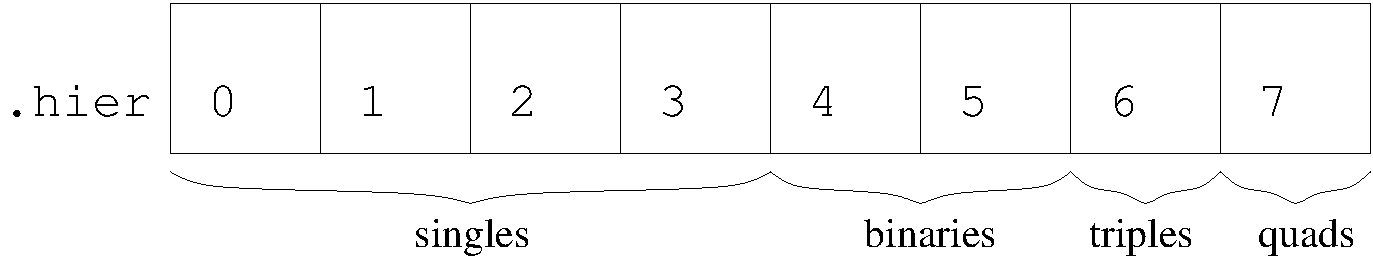
\includegraphics[scale=0.3]{dot_hier_flat.pdf}
    \caption{The element {\tt .hier} of the {\tt fb\_hier\_t} data type is an array
      of {\tt fb\_obj\_t}s.  This is an example for a {\tt fb\_hier\_t} initialized
      with 4 stars.\label{fig:dot_hier_flat}}
  \end{center}
\end{figure}

\begin{figure}
  \begin{center}
    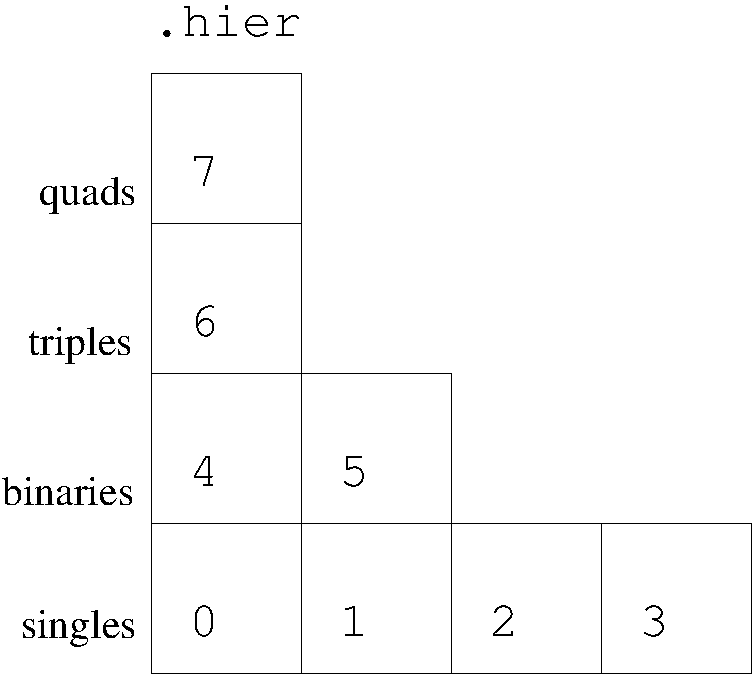
\includegraphics[scale=0.3]{dot_hier_arranged.pdf}
    \caption{It is often convenient to think of the {\tt .hier} element
      as arranged in a sort of pyramid.\label{fig:dot_hier_arranged}}
  \end{center}
\end{figure}

As you may have already guessed, the stars actually ``sit'' in memory in the single star slots.
Each higher order hierarchy contains orbital properties and points (literally, in the C sense) to 
two lower order hierarchies.  For example, a triple would point to a binary and a single star, and contain
the orbital properties of the ``outer'' binary.  The binary it points to would contain the 
``inner'' orbital properties, and point to two single stars.  This is shown on the right side of
Fig.\ \ref{fig:obj_and_hier}, with single stars shown as filled circles and higher order hierarchies
shown as open circles.  Note that by construction, gravitational hierarchies are represented
by binary trees in \Fewbody.  Thus each {\tt fb\_obj\_t} can either point to two lower order 
{\tt fb\_obj\_t}s, or {\em no} {\tt fb\_obj\_t}s (each pointer set to {\tt NULL}).  
This means we can't represent the stable figure-eight orbit \citep{2000MNRAS.318L..61H}.  Since one has never 
been observed in nature and the theoretically expected formation rate is incredibly low, this 
is an approximation that seems safe.

\begin{figure}
  \begin{center}
    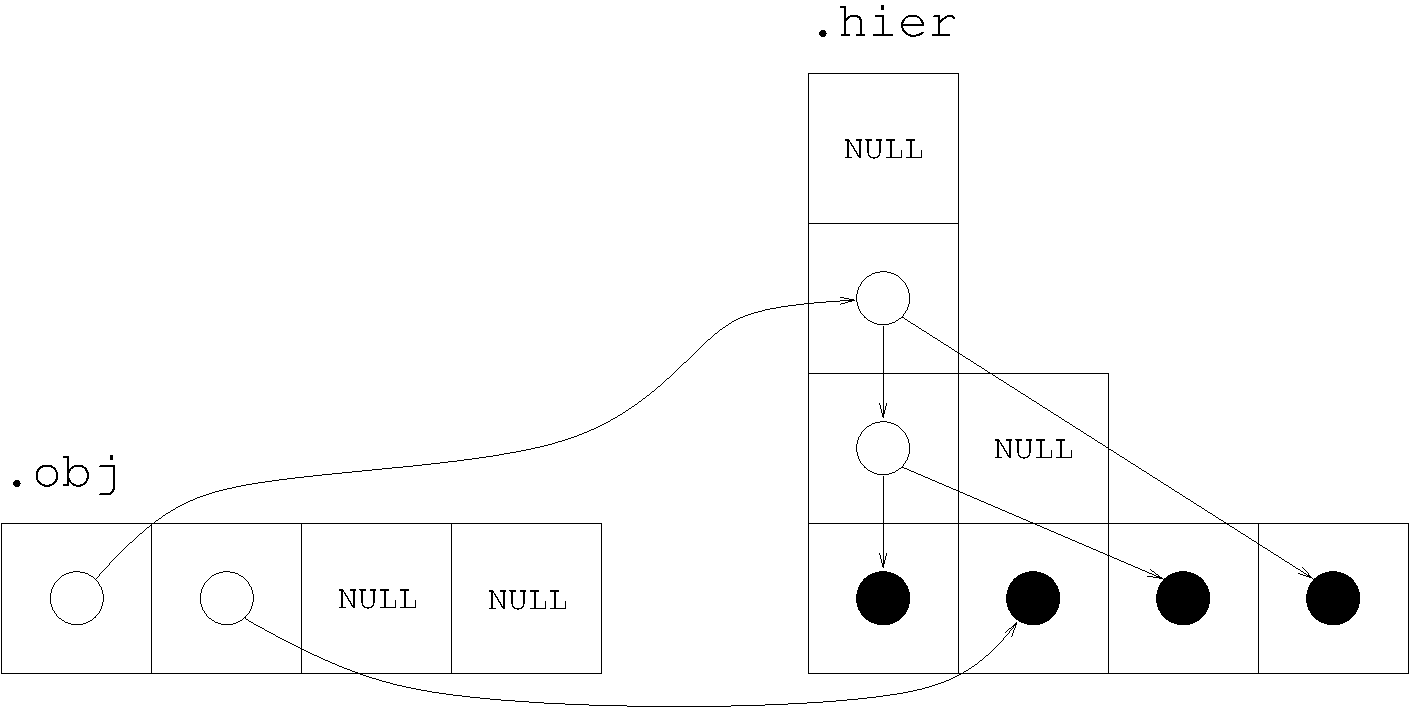
\includegraphics[scale=0.3]{obj_and_hier.pdf}
    \caption{The stars are arranged in hierarchies, as shown on the right side of this
      figure.  The {\tt .obj} element of {\tt fb\_hier\_t} is an array that points to the 
      separate hierarchies in the system.  Each hierarchy pointed to in {\tt .obj} is 
      gravitationally {\em unbound} from the other hierarchies.  So in this example
      there are separately a triple and a single star that are unbound from each other.
      \label{fig:obj_and_hier}}
  \end{center}
\end{figure}

So far we have described only how the data structures can be arranged in \Fewbody, but not how \Fewbody\
actually does things.  When the {\tt fewbody()} function returns (more of that later), 
the {\tt .hier} is organized as the set of gravitational hierarchies that are unbound from 
each other.  So if a system of 4 stars is arranged as a bound triple and a single star that
are not bound to each other, it will look like the right side of Fig.\ \ref{fig:obj_and_hier}.
For convenience, {\tt fb\_hier\_t} contains an element {\tt .obj} that points to the separate
hierarchies in {\tt .hier}.

For completeness, let's go through all the pieces of the {\tt fb\_hier\_t} data type.
(You can follow along by looking at {\tt fewbody.h} from your source distribution.)
We've already described {\tt .hier}, {\tt .hi}, and {\tt .obj}.  {\tt .narr[n]} gives
the number of hierarchies of order $n$.  For example, for Fig.\ \ref{fig:obj_and_hier},
we have {\tt .narr[2]=1}, {\tt .narr[3]=1}, and {\tt .narr[4]=0}.  {\tt .nstar} gives
the current number of single stars, and would be 4 in this example.  {\tt .nobj} gives
the number of used elements in the {\tt .obj} array, and would be 2 in this example.
Finally, {\tt .nstarinit} is the number of stars that was used to initialize the 
{\tt fb\_hier\_t}.  {\tt .nstar} can be less than {\tt .nstarinit} if stars have
collided and merged.

Let's talk about the {\tt fb\_obj\_t} data type.  This is the data type that makes up 
{\tt .hier} and {\tt .obj} in {\tt fb\_hier\_t}.  It represents either a node or a leaf in
a gravitational binary tree.  Since physically it represents a star or a bound pair of somethings,
it's name is meant to evoke a generic gravitational ``object''.  If you take a look
at the definition of this data type in {\tt fewbody.h}, you'll see this structure has 
many elements.  Most notably, it has an array of two pointers to other {\tt fb\_obj\_t}s 
in the element {\tt .obj}.  If these pointers are {\tt NULL} the object is a single star.
If they both point to something it's a bound pair of somethings.  (If only one pointer
is set something went terribly wrong.)  The total number of stars contained in all lower
levels of the tree can be found in the element {\tt .n}.  It should be evident directly
from the data type definition that there are elements that describe dynamical properties (mass,
position, velocity), single star specific quantities (radius, internal energy, internal
angular momentum), and quantities that are only used when the {\tt fb\_obj\_t} represents
a bound pair (semi-major axis, eccentricity, angular momentum unit vector, Runge-Lenz vector,
orbital reference time, and mean anomaly).  {\tt .ncoll} is an element specific to single stars,
and tells you how many stellar mergers this star represents.  If it is 1 there have been no 
mergers, if it is $n$ there have been $n-1$ mergers.  {\tt .ncoll} is the used length
of the {\tt .id} array, which contains the unique user-assigned identifiers of all
the stars that have merged in this star.

%%%%%%%%%%%%%%%%%%%%%%%%%%%%%%%%%%%%%%%%%%%%%%%%%%%%%%%%%%%%%%%%%%%%%%%%%%%%%%%
\section{Basic Usage}\label{sec:basicusage}
Although the source for the command line utilities that come with \Fewbody\ may appear complicated,
there are in fact just a few things that need to be set to have \Fewbody\ evolve
a system.  First, a {\tt fb\_hier\_t} has to be initialized with the desired number
of stars; let's say we have one called {\tt myhier}.  Then the properties of the 
single stars have to be set in {\tt myhier.hier}.  Note that the units used (for 
lengths, masses, time, etc.) can be any units you like, as long as it is a system of units
in which the gravitational constant $G=1$.  You may make use of the {\tt fb\_units\_t}
data type for this purpose, if you wish.  Next, you must set some parameters
in a {\tt fb\_input\_t}---we'll call it {\tt myinput}---which include integration
parameters and tolerances, and the stopping time of the calculation.  Then you're 
ready to run \Fewbody.  If we call our time variable {\tt t}, then we run \Fewbody\
like this:
\begin{verbatim}
  myretval = fewbody(myinput, &myhier, &t);
\end{verbatim}
where {\tt myretval} will contain output information from \Fewbody\ in the {\tt fb\_ret\_t}
type.  The time {\tt t} will be updated with the time at the end of the calculation, and {\tt myhier}
will be returned with the gravitational organization of the $N$-body system at the end of
the calculation.  As we will see below, {\tt myhier} can be traversed using a variety of techniques
to get the hierarchical organization of the system, extract values, etc.

%%%%%%%%%%%%%%%%%%%%%%%%%%%%%%%%%%%%%%%%%%%%%%%%%%%%%%%%%%%%%%%%%%%%%%%%%%%%%%%
\section{An Example}\label{sec:example}
How about an example showing the minimum amount of setup needed to start a \Fewbody\
run?  For this example, let's assume we have 5 stars that we want to initialize
with given positions and velocities, and see what the outcome is.
Units are often a subtle and tricky thing.  Let's initialize everything in cgs
units, then define our units with a routine we write.  \Fewbody\ will do the normalization
for us.  I assume you're familiar enough with C to properly prototype all functions, 
include the appropriate headers, etc.  Here we go:

\verbatimtabinput[8]{simple.c}

And here is the output of this code on my machine (it may differ from machine to machine due
to round-off error and the inherent chaos in the $N$-body problem):

\begin{verbatim}
encounter NOT complete.
final configuration:  nstar=5 nobj=1:  [[[0 2] [1 3]] 4]  (quintuple)
t_final=10000.9 (711.854 yr)  t_cpu=0.47 s
DeltaL/L0=3.60588e-08  DeltaL=1.08282e-09
DeltaE/E0=-2.94682e-07  DeltaE=3.94031e-09
Rmin=0.000125687 (0.0270158 RSUN)  Rmin_i=2  Rmin_j=4
Nosc=0 (non-resonance)
orbital parameters of outermost binaries:
j=0  a=19.1876 AU  e=0.744792
\end{verbatim}

My hope is that the code example above answers more questions than it raises.  It may seem verbose,
but I encourage you to read through it line by line, as I have tried to comment the important
parts.

%%%%%%%%%%%%%%%%%%%%%%%%%%%%%%%%%%%%%%%%%%%%%%%%%%%%%%%%%%%%%%%%%%%%%%%%%%%%%%%
\section{Another Example}\label{sec:anotherexample}
Suppose you want to do something more advanced with \Fewbody.  Suppose you 
have evolved a system with a fairly large number of stars, and want to find the
relative inclination in any triples that result.  Here's how you might do something
like this:

\begin{verbatim}
for (j=0; j<hier.nobj; j++) {
  if (hier.obj[j]->n == 3) {
    /* determine which element is inner binary */
    if (hier.obj[j]->obj[0]->n == 1) {
      is = 0;
      ib = 1;
    } else {
      is = 1;
      ib = 0;
    }

    /* calculate outer angular momentum  */
    fb_cross(hier.obj[j]->obj[0]->x, hier.obj[j]->obj[0]->v, l0);
    fb_cross(hier.obj[j]->obj[1]->x, hier.obj[j]->obj[1]->v, l1);

    for (i=0; i<3; i++) {
      Lout[i] = hier.obj[j]->obj[0]->m * l0[i] + hier.obj[j]->obj[1]->m * l1[i];
    }

    /* calculate inner angular momentum */
    fb_cross(hier.obj[j]->obj[ib]->obj[0]->x, hier.obj[j]->obj[ib]->obj[0]->v, l0);
    fb_cross(hier.obj[j]->obj[ib]->obj[1]->x, hier.obj[j]->obj[ib]->obj[1]->v, l1);

    for (i=0; i<3; i++) {
      Lin[i] = hier.obj[j]->obj[ib]->obj[0]->m * l0[i] + 
               hier.obj[j]->obj[ib]->obj[1]->m * l1[i];
    }

    /* acos returns a value between 0 and PI */
    inc = acos(fb_dot(Lin, Lout)/(fb_mod(Lin)*fb_mod(Lout)));
    fprintf(stderr, "j=%d  inc=%g radians\n", j, inc);
  }
}
\end{verbatim}

%%%%%%%%%%%%%%%%%%%%%%%%%%%%%%%%%%%%%%%%%%%%%%%%%%%%%%%%%%%%%%%%%%%%%%%%%%%%%%%
\section{The Functional Interface}\label{sec:functional}
By request, I have created a rudimentary functional interface to \Fewbody,
which uses function calls to access and set elements of a {\tt fb\_hier\_t},
traverse its structure, etc.  The functions are essentially shortcuts to
using the arrays defined in the data types.  Here's one self-explanatory example 
from {\tt fewbody\_ui.c}:

\begin{verbatim}
int fbui_make_pair(fb_obj_t *parentobj, fb_obj_t *obj1, fb_obj_t *obj2)
{
  parentobj->obj[0] = obj1;
  parentobj->obj[1] = obj2;
  return(0);
}  
\end{verbatim}

And you use it like this:

\begin{verbatim}
  fbui_make_pair(fbui_hierarchy_binary(&hier, 0),
                 fbui_hierarchy_single(&hier, 1),
                 fbui_hierarchy_single(&hier, 2));
\end{verbatim}

I have created a full example of how to use the functional interface in
the file {\tt binsingle\_simple.c}.  Please have a look at it to see
how this interface is used in practice.  In it you will also notice some 
other useful utilities provided by \Fewbody, including a routine to randomly
orient a binary (when you don't care about orientation, phase, etc., and want
to average over them in an ensemble of scattering calculations), and a routine
to bring a pair of objects in from infinity along a hyperbolic orbit to the point
where you want to start numerical integration (this is very useful for scattering
experiments).

%%%%%%%%%%%%%%%%%%%%%%%%%%%%%%%%%%%%%%%%%%%%%%%%%%%%%%%%%%%%%%%%%%%%%%%%%%%%%%%
\section{Appendix}\label{sec:appendix}
For completeness, this section provides details on \Fewbody\ data types, in the form
of tables.  The other \Fewbody\ data types are documented fairly well in {\tt fewbody.h}.


\begin{figure}
  \begin{tabular}{ | l | p{10cm} |}
    \hline
    {\tt .ncoll}& length of {\tt .id} array\\
    {\tt .id}& array of stellar ids\\
    {\tt .idstring}& object id in string form\\
    {\tt .m}& mass\\
    {\tt .R}& radius (stars only)\\
    {\tt .Eint}& internal energy (stars only)\\
    {\tt .Lint}& internal angular momentum (stars only)\\
    {\tt .x}& position vector\\
    {\tt .v}& velocity vector\\
    {\tt .n}& number of leaves below and including this node in tree\\
    {\tt .obj}& array of two pointers to child nodes\\
    {\tt .a}& semi-major axis (bound pairs only)\\
    {\tt .e}& eccentricity (bound pairs only)\\
    {\tt .Lhat}& angular momentum unit vector (bound pairs only)\\
    {\tt .Ahat}& Runge-Lenz vector (bound pairs only)\\
    {\tt .t}& orbital reference time (bound pairs only)\\
    {\tt .mean\_anom}& orbital mean anomaly (bound pairs only)\\
    \hline
  \end{tabular}
  \caption{{\tt fb\_obj\_t}, the basic data type for stars and bound pairs of somethings.}
\end{figure}

\begin{figure}
  \begin{tabular}{ | l | p{10cm} |}
    \hline
    {\tt .nstarinit}& number of stars used to initialize {\tt fb\_hier\_t}\\
    {\tt .nstar}& current number of stars\\
    {\tt .nobj}& number of separate, bound hierarchies---used length of {\tt obj} array\\
    {\tt .hi}& array of first indices for a given hierarchy order in {\tt .hier}\\
    {\tt .narr}& array containing number of hierarchies of given order\\
    {\tt .hier}& array of {\tt fb\_obj\_t}s holding gravitational organization of system\\
    {\tt .obj}& array of pointers to separate, bound hierarchies in {\tt .hier}\\
    \hline
  \end{tabular}
  \caption{{\tt fb\_hier\_t}, the basic data type for gravitational hierarchies.}
\end{figure}

%%%%%%%%%%%%%%%%%%%%%%%%%%%%%%%%%%%%%%%%%%%%%%%%%%%%%%%%%%%%%%%%%%%%%%%%%%%%%%%
\acknowledgements

%%%%%%%%%%%%%%%%%%%%%%%%%%%%%%%%%%%%%%%%%%%%%%%%%%%%%%%%%%%%%%%%%%%%%%%%%%%%%%%
\bibliographystyle{apj}
\bibliography{apj-jour,main}

\end{document}
